\addvspace{1cm}
\subsection{Anwendung der Laplace Transformation in der Systemtheorie und Regelungstechnik}

Mithilfe der Laplace Transformation lassen sich Systeme und ihre Funktionen aus dem Zeitbereich im Bildbereich (Frequenzbereich) darstellen. Dazu ein Beispiel aus der Elektrotechnik:

\vspace{1em}  % vertikaler Abstand zwischen Elementen

\noindent
\begin{minipage}[t]{0.35\textwidth}
    \textbf{Ohmscher Widerstand}\\[0.5ex]
    \(
    \begin{aligned}
    u_R(t) &= R\, \dot{i}_R(t) \\
    \dot{i}_R(t) &= \frac{1}{R} u_R(t)
    \end{aligned}
    \)
\end{minipage}%
\hfill
\begin{minipage}[t]{0.3\textwidth}
    \vspace*{-0.3ex} % optionales Feintuning
    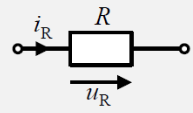
\includegraphics[width=0.8\textwidth]{Anlagen/ohmscher_Widerstand.png}
\end{minipage}%
\hfill
\begin{minipage}[t]{0.25\textwidth}
    \raggedleft
    \vspace*{-0.3ex} % optional, damit Quelle auch oben beginnt
    \cite{manual1}
\end{minipage}
\vspace{1.5em}
\noindent
\begin{minipage}[t]{0.35\textwidth}
    \textbf{Induktivität}\\[0.5ex]
    \(
    \begin{aligned}
    i_L(t) &= \frac{1}{L} \int_0^t u_L(\tau) \, d\tau + i_{L0} \\
    u_L(t) &= L \frac{d i_L(t)}{dt} \quad \text{mit} \quad i_L(0) = i_{L0}
    \end{aligned}
    \)
\end{minipage}%
\hfill
\begin{minipage}[t]{0.3\textwidth}
    \vspace*{-0.3ex}
    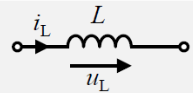
\includegraphics[width=0.8\textwidth]{Anlagen/Spule.png}
\end{minipage}%
\hfill
\begin{minipage}[t]{0.25\textwidth}
    \raggedleft
    \vspace*{-0.3ex}
    \cite{manual1}
\end{minipage}

\vspace{1.5em}
\noindent
\begin{minipage}[t]{0.35\textwidth}
    \textbf{Kapazität}\\[0.5ex]
    \(
    \begin{aligned}
    u_C(t) &= \frac{1}{C} \int_0^t i_C(\tau) \, d\tau + u_{C0} \\
    i_C(t) &= C \frac{d u_C(t)}{dt} \quad \text{mit} \quad u_C(0) = u_{C0}
    \end{aligned}
    \)
\end{minipage}%
\hfill
\begin{minipage}[t]{0.3\textwidth}
    \vspace*{-0.3ex}
    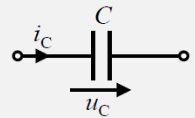
\includegraphics[width=0.8\textwidth]{Anlagen/Kondensator.png}
\end{minipage}%
\hfill
\begin{minipage}[t]{0.25\textwidth}
    \raggedleft
    \vspace*{-0.3ex}
    \cite{manual1}
\end{minipage}

\vspace{1.5em}
\noindent
\begin{minipage}[t]{0.35\textwidth}
    \textbf{Ideale Spannungsquelle}\\[0.5ex]
    \(
    u_0(t) = f(t)
    \)
\end{minipage}%
\hfill
\begin{minipage}[t]{0.3\textwidth}
    \vspace*{-0.3ex}
    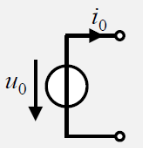
\includegraphics[width=0.8\textwidth]{Anlagen/Spannungsquelle.png}
\end{minipage}%
\hfill
\begin{minipage}[t]{0.25\textwidth}
    \raggedleft
    \vspace*{-0.3ex}
    \cite{manual1}
\end{minipage}

\vspace{1.5em}
\noindent
\begin{minipage}[t]{0.35\textwidth}
    \textbf{Ideale Stromquelle}\\[0.5ex]
    \(
    i_0(t) = f(t)
    \)
\end{minipage}%
\hfill
\begin{minipage}[t]{0.3\textwidth}
    \vspace*{-0.3ex}
    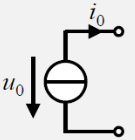
\includegraphics[width=0.8\textwidth]{Anlagen/Stromquelle.png}
\end{minipage}%
\hfill
\begin{minipage}[t]{0.25\textwidth}
    \raggedleft
    \vspace*{-0.3ex}
    \cite{manual1}
\end{minipage}

\addvspace{1cm}
\paragraph{Beispielaufgabe:}

Für folgendes elektrisches Netzwerk soll die Übertragungsfunktion aufgestellt werden:


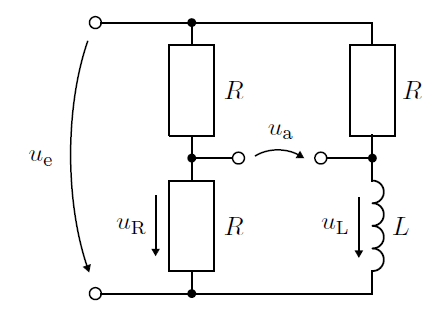
\includegraphics[width= 0.5\textwidth]{Anlagen/System_mit_1_E_Speicher.png}

Die Netzwerkanalyse findet dabei nach den Kirchhoffschen Regeln aus der Elektrotechnik statt und die Laplace Transformation nach den Regeln der Linearität (9) (Ohmscher Widerstand, Spannungsein- und -ausgang) und Ableitung (Induktivität) (14).
\[
u_R = \frac{R}{R + R} u_e = \frac{1}{2} u_e
\]

\[
\mathcal{L} : \quad U_R(s) = \frac{1}{2} U_e(s)
\]

\[
U_L(s) = \frac{L s}{R + L s} U_e(s)
\]

\[
U_a(s) = U_R(s) - U_L(s) = \left( \frac{1}{2} - \frac{L s}{R + L s} \right) U_e(s) 
= \frac{\frac{1}{2}(R + L s) - L s}{R + L s} U_e(s)
\]

\[
G(s) = \frac{U_a(s)}{U_e(s)} = \frac{\frac{1}{2} R - \frac{1}{2} L s}{R + L s} 
= \frac{1}{2} \cdot \frac{1}{R} \left( 1 - \frac{L}{R} s \right) 
= \frac{1}{2} \cdot \left( \frac{1 - \frac{L}{R}s}{1 + \frac{L}{R}s} \right) 
= \frac{1}{2} \cdot \frac{1 - \frac{L}{R}s}{1 + \frac{L}{R}s}
\]

\addvspace{1cm}
\textbf{Verknüpfung von Übertragungssystemen}

Im vorangegangenen Beispiel wurde ein erstes Beispiel gegeben, das ein Übertragungssystem darstellt. Sind nun mehrere Übertragungssysteme gegeben, für die bereits eine Funktion im Bildbereich bekannt ist, können sie miteinander verknüpft werden.
Dies kann auf verschiedenen Wegen geschehen. Übertragungssysteme können in Reihe, parallel, per Rückkopplung oder auch durch eine Mischung der vorangegangenen Fälle miteinander verknüpft sein.

\paragraph{In Reihe:}

Sind mehrere Übertragungssysteme in Reihe geschaltet, kann man sie über Multiplikation zu einem neuen System zusammenfassen. Dabei ist zwischen zwei Systemen einmal das Ausgangssignal eines Übertragungssystems das Eingangssignal eines anderen \cite[S. 902]{buch1}.

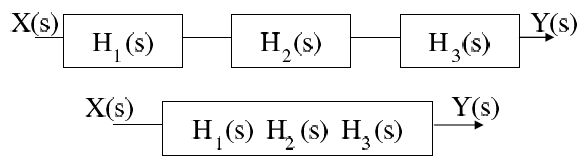
\includegraphics[width= 0.5\textwidth]{Anlagen/Übertragungssysteme_in_Reihe.png}
\cite[S. 902]{buch1}

\paragraph{Parallel:}

Sind Übertragungssysteme parallel zueinander, dann werden sie miteinander addiert, um sie zusammenzufassen.

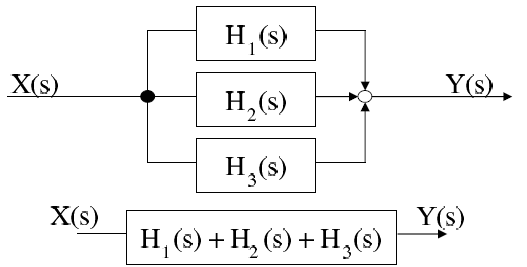
\includegraphics[width= 0.5\textwidth]{Anlagen/Übertragungssysteme_parallel.png}
\cite[S. 902]{buch1}

\paragraph{Rückkopplung:}

Vom transformierten Eingang X(s) wird bevor er auf den Ausgang wirken kann, die Rückkopplung abgezogen.

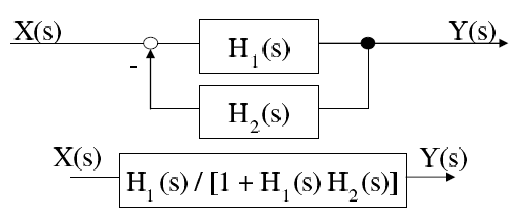
\includegraphics[width= 0.5\textwidth]{Anlagen/Übertragungssysteme_Rückkopplung.png}

Herleitung:
\begin{align*}
    Y(s) &= H_1(s) \left[ X(s) - Y_R(s) \right] 
    = H_1(s) \left[ X(s) - H_2(s) Y(s) \right] \\
    &\Leftrightarrow \left[ 1 + H_1(s) H_2(s) \right] Y(s) = H_1(s) X(s).
    &\Leftrightarrow \frac{Y(s)}{X(s)} = \frac{H_1(s)}{1 + H_1(s) H_2(s)}.
\end{align*}
    \cite[S. 902]{buch1}
    

